
\selectlanguage{english}
\def\<#1>{\textit{#1}}

\chapter{Hash Tables}
\section{Introduction}

Hash Tables are a fundamental data structure that provides fast store and lookup operations, and it is used in various programming applications. The ability ,for example ,to create sets and quickly perform searches on them, depends on the efficiency of the underlying Hash Table. For this reason, many algorithms and approaches, both sequential and concurrent have been put forward, each with its own distinctive strengths and weaknesses. 

The purpose of a Hash Table is to efficiently associate a given value with a key and use that key to rapidly store or search that value among other values. It usually consists of an array or list of buckets, which can hold one or more values, as well as a hash function that maps a value on the table.

Ideally,  every different values will hash to different buckets, making it easy to insert and search them, However, it is improbable that there will be no collisions, in fact for a large number of operations we expect collisions to be quite common. For the purpose of avoiding collisions, one must consider the size of the hash table (more buckets  means more ways to distribute the keys) and the hash function ( a hash function that will evenly distribute keys among the available buckets will reduce collisions). Even so, collisions are unavoidable, and the way they are handled is one the most important factor among the various implementations.

\subsection{Collision Resolution}

Hash tables can be divided into two main categories: Closed Addressing and Open Addressing.

%add some bullets here

Closed addressing hash tables allow more than one values to be stored on the same bucket. This is usually implemented by attaching a linked list at the start bucket , and each new value is added on the list. The length of the list  must be kept bellow a constant number (called load factor) , to keep operations on the list fast. This way the average lookup / insertion time is dependent only on load factor. It is common to keep the list ordered , which reduces the average lookup time in half. This is an easy to implement data structure and it has been proven to perform well in practice.

Open addressing hash tables allow no more than a single value per bucket. When a collision is detected, the buckets are traversed in order to find an empty bucket to store the new value, even though it’s hash value does not correspond to that bucket. The sequence according to which the buckets are traversed is typically:

\begin{enumerate}
	\item Linear probing, where an empty bucket is searched within a given number of steps from the mapping bucket
	\item Quadratic probing, where the buckets is searched at increasingly bigger intervals, according to successive values of a quadratic polynomial. 
	\item Double hashing, where interval is the outcome of a new hash function.
\end{enumerate}
% kapoia sxhmata edw

 Some other important techniques used in resolving conflicts in open addressing hash tables is cuckoo hashing and hopscotch. Cuckoo hashing, as explained later in detail, employs a second , or more hash functions. The value is first hashed using the first hash function  and if it corresponds to an non-empty bucket the second hash function is used. If both buckets are empty, then one of the two previously hashed values is evicted and then hashed again using the other hash function, possibly triggering a series of evictions until all values are hashed.

%sxhma gia cuckoo hashing 

Hopscotch hashing combines linear probing and cuckoo hashing. First , buckets are traversed until an empty bucket is found. If that bucket is in the neighborhood of the initially mapped bucket, the value is placed there, just as in linear probing. If the empty bucket is outside the neighborhood, values are moved in a sequence of hops, effectively moving the empty slot closer and closer to the neighborhood of the initial bucket. An example is shown at figure \ref{fig:hopscotch_hashing}.

%sxma gia hopscotch hasing
\begin{figure}
 \centering
  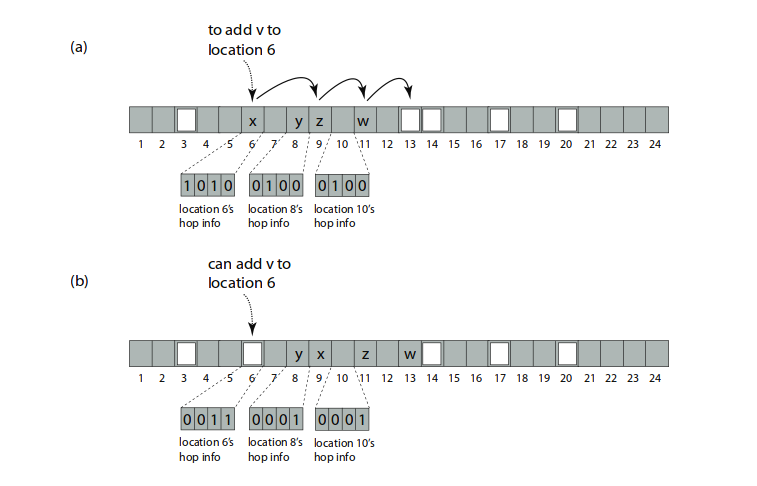
\includegraphics[scale=0.5]{hopscotch_hashing.png}
\caption{Example of an insertion in hopscotch hashing. Here we try to insert value 6 and the first empty bucket is found at index 13, outside the neighbourhood of bucket 6. We then find out that w an index 11 can be displaced to the empty bucket and we place it there. Now the empty bucket is at index 11 wich is still far from 6. Subsequently, by switching places with buckets 9 and 6, the empty bucket is finally at index 6 and the new value can be inserted }
\label{fig:hopscotch_hashing}
\end{figure}


\subsection{Resizing}

Resizing is important to maintain constant average insertion and lookup time. In closed addressing algorithms, buckets may become too full, making their traversal slow, while in open addressing algorithms, the table may become too full to easily  find empty buckets . In either case, the size of the table needs to be expanded and all the values from the old, small hash table must be transferred to the new bigger one. This can be done by rehashing every value of the old table to the new one (possibly causing a high delay which may not be acceptable in a real time application) or  incrementally , by moving every new inserted value to the new table , along with a few elements from the old table each time, until the old table is empty.

\subsection{Concurrent hash tables}

In a multiprocessor environment it is quite common for multiple threads to require concurrent access to the same hash table. Access on disjoin locations on the hash tables, suggests hash tables are may allow a much higher level of concurrency, compared to FIFO queues as studied above. However, keeping the data structure fast and consistent despite contention, introduces many challenges and many diverse concurrent algorithms have been proposed to face them.
   
% edw tha moune oi alles ylopoihseis

\section{ Locking Approaches}

We start by implementing the hash table as a table of nodes, with each node being the head of a simple linked list that we keep ordered. We protect the table with a simple spinlock. Each thread needs to acquire the spinlock before performing any operation ( insert, lookup or delete). 

In order to ensure that every operation takes constant time, we need to keep the average number of items in every link list bellow a minimum. This is done by resizing the table , according to a certain policy. The resizing mechanism may trigger when the number of buckets that have grown beyond a certain threshold is large, or when the total ratio of inserted elements to the number of buckets exceeds a threshold. To perform the resize operation, a thread acquires the lock, checks if another thread has already resized the table and if not, proceeded to allocate a new table twice as big as the old one and then rehash every value from the old table into the new one.

The global lock mechanism is simple to implement but it introduces a sequential bottleneck and performance is low, as shown in figure \ref{hashes_global_perf}. All threads spin on the same lock, even they are trying to access disjoint locations on the table . Moreover , since the critical section inside the lock is very small, the overhead of acquiring and releasing the lock becomes a large proportion of runtime.

\begin{figure}
 \centering
  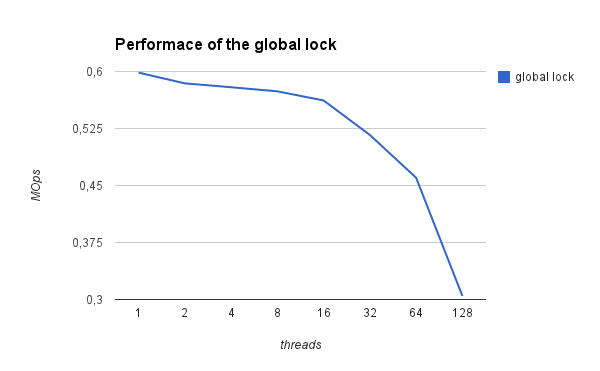
\includegraphics[scale=0.7]{hashes_global_perf.png}
\caption{The performance of the naive global lock approach}
\label{hashes_global_perf}
\end{figure}

We then try to permit more concurrency by used a fixed number of locks , instead of a single one. We introduce an array of spinlocks with length L, with each lock protecting a number of buckets. We determine which lock is responsible for each bucket by simply mapping the index of the bucket on the array of locks. As the table grows, the number of locks remains the same ,so each lock is responsible for more buckets, as shown in figure \ref{striped_hash_set}.

%sxhma apo to vivlio tou shavit
\begin{figure}
 \centering
  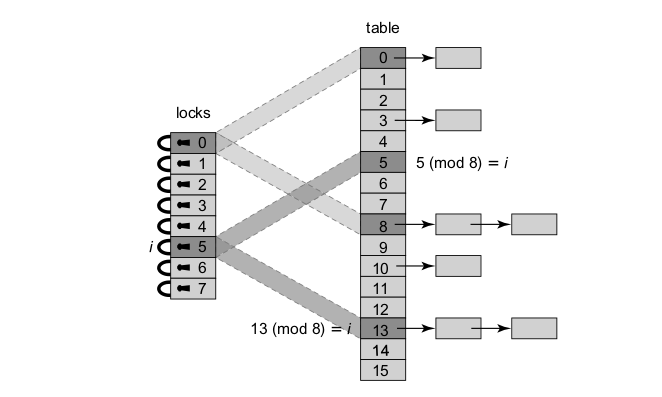
\includegraphics[scale=0.5]{striped_hash_set.png}
\caption{A representation of the striped hash set}
\label{striped_hash_set}
\end{figure}


Having more than one locks means more than one threads can proceed  successfully and this results to less contention, more concurrency and improved performance. Increasing the number of locks , closer and closer to the number of buckets, seems to improve throughput and refuce latecny , as depicted in figures \ref{hashes_striped_through} and \ref{hashes_striped_latency}. However, if we want to keep the number of locks equal to the number of buckets, as the table increases in size, we need to be able to resize the lock array as well, which is not straight forward.

\begin{figure}
 \centering
  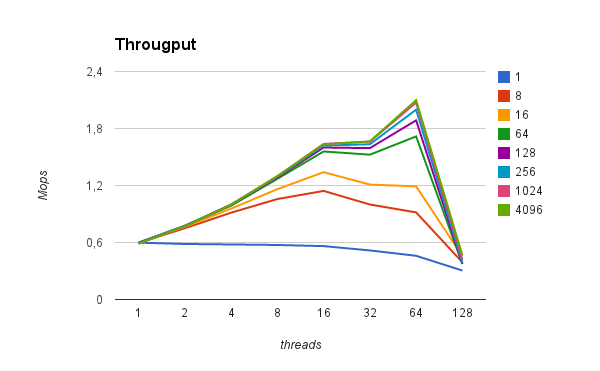
\includegraphics[scale=0.7]{hashes_striped_through.png}
\caption{Throughput for various numbers of locks}
\label{hashes_striped_through}
\end{figure}

\begin{figure}
 \centering
  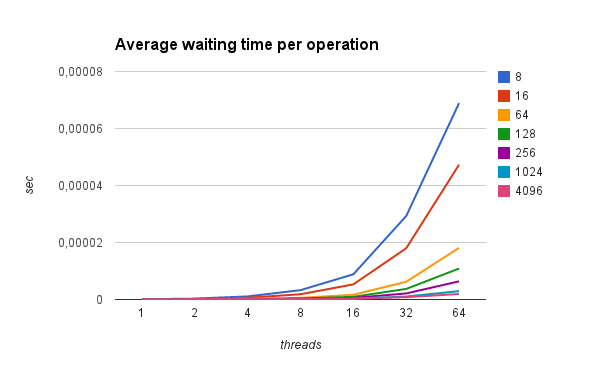
\includegraphics[scale=0.7]{hashes_striped_latency.png}
\caption{Latency for various numbers of locks}
\label{hashes_striped_latency}
\end{figure}
For this reason we then try to implement a refinable locking scheme, where locks can be dynamically increased to match the number of buckets. Here, we require mutual exclusion between resizing and updating, so we introduce a marked field owner, containing the id of the thread that is currently resizing. When a thread is trying to resize, it first atomically sets the mark bit and writes its id in the owner field. It then waits until no more updates are being performed(e.g. all the locks are unlocked). That way, all other threads that are trying to update, will find the marked bit of the owner value set and will not proceed to take any lock. The thread is now free to resize the table and the lock array, rehash every value into the new table and unset the marked bit. In this implementation, we also allow lookups to first search the value without taking a lock. This allows to sometimes successfully perform lookups, even during resizing. If the value is found, lookup returns that value. If not, it might be possible that the value was inserted but the thread could not access it yet, so the thread tries searching again, this time holding the lock. 

The outline of the function used by every thread to acquire a lock is shown here, where we can see how the when the mark bit of the owner field is set, no one can acquire any locks.

\begin{lstlisting}[caption={Acquiring the lock for the refinable hash table }]

void acquire(HashTable_t T , int x){
	
	me =  current thread index
	while (1){
		do{
			<who, mark> = owner
		}while (mark && who != me)
		
		Locks[] oldLocks = locks
		lock the apropriate lock on oldLocks array
		<who, mark> = owner
		if ((!mark || (who == me)) && locks = oldLocks)
			return
		else 
			unlock the lock from oldLocks array 
	}
}

\end{lstlisting}

The result is an increase in performance, because we exploit the finer grained syncronization. However, this imporovement comes with the cost of slower resizing. Increasing the number of locks means that we need more time to allocate the extra locks and more time to wait until all locks are free. The extra amount of time introduced is shown in figure \ref{hashes_refinable_resize}. In fact, figure \ref{hashes_refinable_stop_resizing} suggests that it would be better to stop resizing the locks array after a certain point.
 
\begin{figure}
 \centering
  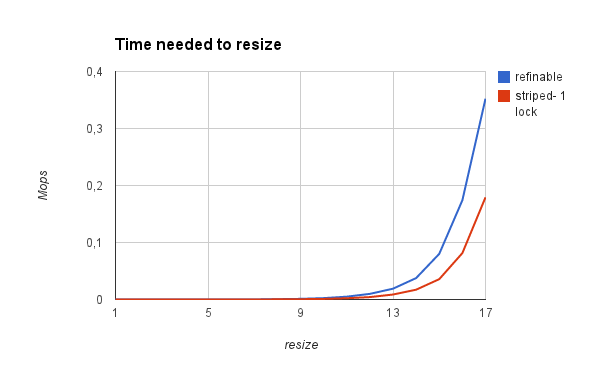
\includegraphics[scale=0.7]{hashes_refinable_resize.png}
\caption{The amount of time needed for every resize}
\label{hashes_refinable_resize}
\end{figure}

\begin{figure}
 \centering
  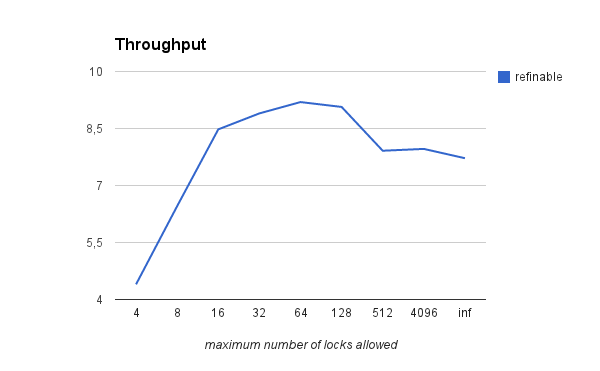
\includegraphics[scale=0.7]{hashes_refinable_stop_resizing.png}
\caption{Setting a maximum granuality level affects performance }
\label{hashes_refinable_stop_resizing}
\end{figure}

\section { Split Ordered List}

All the above mentioned algorithms use locks to enforce synchronization and therefore inherit all the disadvantages of blocking algorithms such as low performance when the number of threads exceeds the number of available cores. Moreover, these algorithms perform resizing in a "stop -the - world" manner, meaning that a single thread resizes the table and during that time no other thread can proceed. We now focus on a lock free algorithm  by  Shalev and Shavit  \cite{split_ordered} ,that uses atomic operations for synchronization and the hash table can grow incrementally without having to rehash any value or introduce a thread barrier.

The algorithm is based on a lock-free linked list , implemented by Michael \cite{lock_free_list} to store the values. The buckets, kept in a single array, are now references to specific nodes in the list, representing the start of the particular bucket, effectively working as short-cuts into the list. As the list grows, we introduce new buckets that split the older ones in half, keeping their size bellow a maximum value. In order to do this however, the list must be kept ordered according to a recursive split order, as described next.

Split ordering is in fact the reverse bit representation of values, kept in ascending order. The goal here is to split each bucket by inserting a new one, without having to rearrange anything else. Figure \ref{split_ordered_1} explains how split ordering achieves just that.

% figure apo th diafania kai exhghsh
\begin{figure}
 \centering
  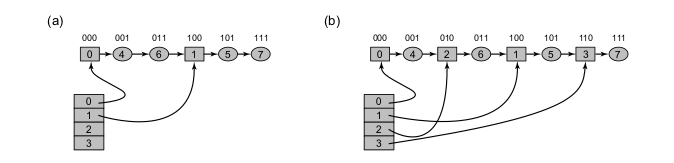
\includegraphics[scale=0.5]{split_ordered_1.png}
\caption{This figure explains how split ordeding manages to effectively split a bucket in half.In part a , the list consists of two buckets. Above each node is it's split-ordered key, which is the reversed bit representation of each value. Square nodes are sentinel nodes, depicting the start of each bucket. When the table capacity grows from 2 to 4 in  part b, two new buckets are inserted, spliting the older one in half}
\label{split_ordered_1}
\end{figure}

There are some extra things to note here that illustrate why this specific type of ordering is the ideal for our need. Imagine a thread trying to search for the value 6 in the hash table depicted in part a. The capacity ( the number of buckets is 2) so values 6 hashes to bucket zero. The thread starts traversing the list and while being at node value 4, a delay occurs. During that delay, capacity is double and a new bucket (bucket 2) is inserted between values 4 and 6, splitting bucket zero in half. As seen above, 2 is prior to 6 according to split ordering, and that mean that traversal well go past 2 and keep looking until it successfully finds the value 6. This depicts a key idea of the algorithm: when the table's capacity is doubled from 2\textsuperscript{i} to 2\textsuperscript{i+1}, a buckets b is split in half and those elements with values k for witch k mod 2\textsuperscript{i+1} =b  remain in bucket b while the others migrate to bucket b + 2\textsuperscript{i}. The algorithm ensures that these two bucket are positioned one after an other, so that in order to split the bucket we don’t really have to move any node around, but instead we only need to let the new bucket start after the first group of items and before the second.

To avoid the case where a node referenced by a bucket is deleted, we use sentinel nodes, inserted at the lists locations pointed to by every bucket. We use the Least Significant Bit of the reversed bit representation to differentiate between normal node and sentinel node and we don not de-allocate these sentinels node during deletion operation, in order to avoid corner cases.

In order to keep track of the load factor, we update a shared variable on every insert/delete operation that depicts the number of values currently stored in the table. If the ratio of inserted values to number of bucket exceeds a certain limit, we double the capacity, thus introducing new available buckets. Note that, in order to avoid complexity, we allocate a large array of buckets in advance. By introducing an extra level of indirection, namely an array of array of buckets, we are able to adaptable increase the maximum number of available buckets if needed.

Figure \ref{split_ordered_2} is an example of how adding a new value in the hash table increases capacity and introduces new buckets.

% figure gia insert apo diafanies kai exhghsh 
\begin{figure}
 \centering
  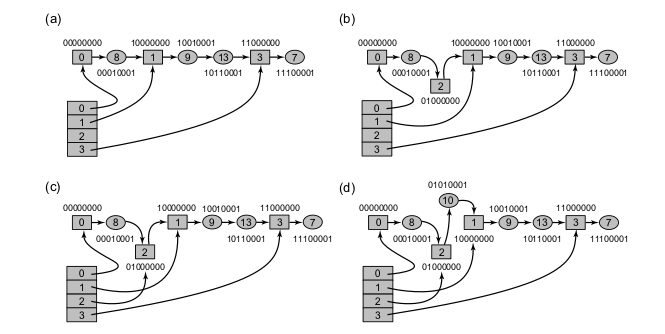
\includegraphics[scale=0.5]{split_ordered_2.png}
\caption{Example of an insertion in the split ordered list. At part a , the bucket 2 is uninitialized. Inserting value 10, initializes the bucket, inserting a sentinel node in the list, before the actuall insertion of 10 at part d}
\label{split_ordered_2}
\end{figure}

Note that unused buckets are uninitialized. The sentinel nodes for each bucket are only inserted when it is actually needed, that is when this buckets holds at least one value. When initializing a bucket, we might also need to recursively initialize other buckets that come before it as shown in figure \ref{split_ordered_3}

% figure gia initialization apo diafanies
\begin{figure}
 \centering
  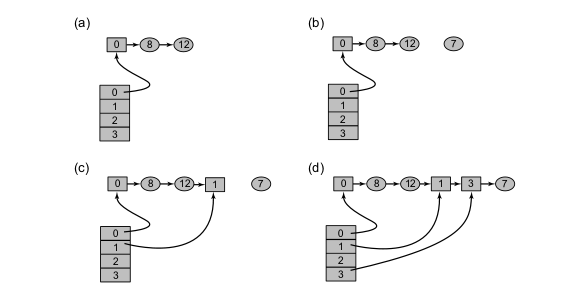
\includegraphics[scale=0.5]{split_ordered_3.png}
\caption{Example of recursive initialization of buckets, before insertion of value 7}
\label{split_ordered_3}
\end{figure}

The insert operations looks very simple, simply initializing the bucket if needed and then insert the split-ordered key in the list starting from the node referenced by the apropriate bucket. Finaly, we check if the capacity need to be doubled. The same outline is followed by the lookup operation.

\begin{lstlisting}[caption={Insert and Loopkup operations of the split ordered algorithm}]

int insert(HashTable_t T, int key){
	node =  allocate new node
	node->key = split_ordered_representation(key)
	bucket = key \% size
	if T[bucket] == uninitialized
		initialize(bucket)
	if (! list_insert(&T[bucket], node)){
		delete node
		return 0
	}
	csize = size
	if (fetch_and_add(&count ,1) / cize > MAX_LOAD)
		CAS(&size,csize, 2 * csize)
	return 1
}

int find(HashTable_t T, int key){
	bucket = key \% size
	if T[bucket] == uninitialized
		initialize(bucket)
	return list_find(&T[bucket], split_ordered_representation(key))
}

\end{lstlisting}

At its lower level, this implementation utilizes a lock free list. Each thread hash a set of three private variables curr, prev and next, each consisting of a pointer to a node, along with a mark bit. These pointers traverse the list to find the appropriate locations for an insertion or deletion and then the thread attempts to atomically modify the list, using Compare And Swap operations

The result, shown in figure \ref{hashes_split_ordered_perf} is a lock free hash table that allows high concurrency, fast operations on the list and most importantly , does not require resizing and rehashing the entire hash table.

\begin{figure}
 \centering
  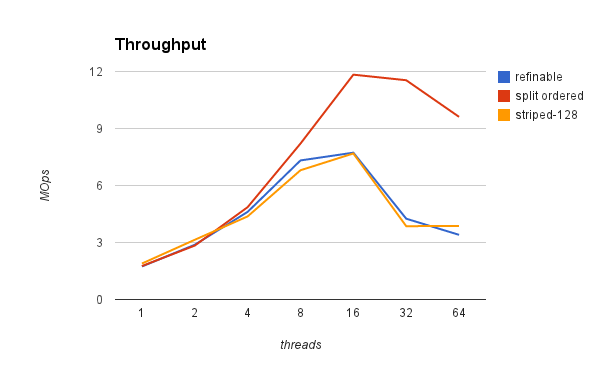
\includegraphics[scale=0.7]{hashes_split_ordered_perf.png}
\caption{Performance of the split ordered algorithm}
\label{hashes_split_ordered_perf}
\end{figure}

\section{Cuckoo Hashing}
\subsection{Sequential version}

We now turn our attention to an open-addressing hash table, called cuckoo hashing. Open-addressing algorithms allow for only one value to be stored at each bucket. In its sequential version, cuckoo hashing uses two arrays of buckets and two hash functions, although it is possible to use only a single array. 

Lookup operations are quite simple. The value is hashed using the first hash function and the corresponding bucket on the first array is checked. If the value is not found, the second hash function is used and the second array is  checked.  If the value its not there either, the lookup operation returns that the value does not exist on the hash table.

The basic idea behind cuckoo hashing is better shown during the insertion operation. We first hash the value using the first hash function and insert it on the appropriate bucket. If that bucket was initially empty, the process is over. If not, the previous value stored in that bucket is evicted, and we then insert it  on the other hash table, using the other hash function, possibly evicting another value in the process and so on, until an empty bucket is found.

% eikona gia cuckoo hashing insertion.. apo pou?
\begin{figure}
 \centering
  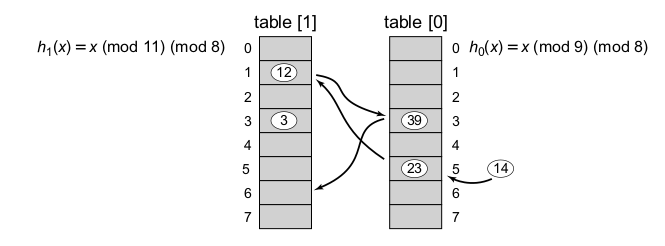
\includegraphics[scale=0.5]{cuckoo_hashing.png}
\caption{Insertion in cuckoo hashing. Trying to insert value 14, we find both apropriate bucket taken by values 3 and 23. Thus, a sequence of displacements is triggered, ending when value 39 is inserted to the previously empty bucket at Table[1][6] }
\end{figure}

The chain of evictions and insertions can grow too long if either the table is too full and no empty buckets can be found easily, or the sequence of displacements form a circle, looping over the same buckets. For this reason, we set an upper limit on the number of evictions triggered by a single insertion. If that limit is exceeded, the table needs to be resized.

There are many variations of the sequential cuckoo hashing algorithms some using more than two different hash function. In general, sequential cuckoo hashing has been proven to work well in practice for a small  to medium load factor.

\subsection{Concurrent version}

In order to implement a concurrent cuckoo hash table, a few changes were maid to the original sequential version. Instead of single element buckets, we use probe sets , whose size is not allowed to grow beyond a certain upper limit. Every set also has a threshold, which is the number of items that can be normally stored inside a bucket. The number of elements stored in a bucket at a given time may exceed the threshold, but the extra elements are marked for eviction and reallocation using the other hash function.

The main principle of the algorithm remains the same. During insertion, the value is added in the set and if the size of the set hash exceeded the threshold, we try to reallocate items using the other hash function and into the other hash table.  In our implementation, we choose to evict the first item on each set, although several other strategies can be chosen instead.

In order to ensure synchronization, we choose to associate every set with its own lock. During any operation (insert, lookup or delete) on a value x, we lock the sets with index h1(x) on table 1 and h2(x) on table 2 accordingly, always in this order, to avoid deadlocks. During resizing, a thread take all the locks on table 1 in ascending order, allocates two new tables, rehashes everything from the old tables to the new ones and releases the locks in the same order. Note that it is possible to implement a striped approach, as discussed in previous implementations, whereas there is a lock-free implementation of cuckoo hashing in the literature \cite{lock_free_cuckoo}.

The basic outline of the insert function is shown bellow.

\begin{lstlisting}[caption={Insert methos of the cuckoo algorithm}]

int insert(HashSet * table, int x){
	acquire the locks on both buckets that x maps to
	h0 = hash0(x)
	h1 = hash1(x)
	i=h=-1
	mustResize = false
	search(x) if found return false
	set0 = table[0][h0]
	set1 = table[1][h1]
	if set0.size < THRESHOLD {
		add(set0, x)
		return true
	}
	else if set1.size < THRESHOLD {
		add(set1, x)
		return true
	}
	else if set0.size < PROBE_SIZE {
		add(set0, x)
		i=0 
		h=h0
	}
	else if set1.size < PROBE_SIZE {
		add(set1, x)
		i=1
		h=h1
	}
	else{
		mustResize = true
	}
	if mustResize{
		resize()	
		insert(T,x)
	else if (! realocate(i,h)){
		resize()
	}
	return true
}
		

\end{lstlisting}

%The result is a concurrent open-addressing algorithm that perform extremely well when the load factor is small enough, especially on workloads that consist mainly of lookups.

In the cuckoo algorithm, search is faster because only two buckets with limited number of items must be checked. However, cuckoo hashing usually requires more than half of the table to be empty in order to perform properly. Moreover, some insertions may cause a realoction chain to loop, forcing the table to resize early, meaning that we cannot easily keep the table from expanding without altering the hash functions. As a result we have bigger tables that are resized more often and during resize, memory allocation is undertaken by a single thread while all the others wait doing nothing.

\begin{figure}
 \centering
  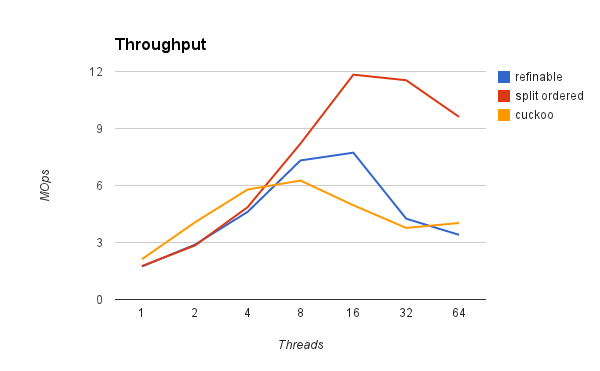
\includegraphics[scale=0.5]{hashes_cuckoo_perf.png}
\caption{Performance of the cuckoo hashing algorithm}
\label{hashes_cuckoo_perf}
\end{figure}

\section{Non Blocking  open addressing}

Last of all, we implemented another open addressing algorithm , introduced by Purchell and Haris \cite{non_blocking_open_addressing} that, unlike cuckoo hashing,  achieves non blocking access by using simple atomic operations.

This algorithm resolves conflicts by using quadratic probing, along the subsequent values of <to polyonymo >.In this implementation, every bucket is accompanied by a probe bound, a value depicting the number of collision on the probe sequence. For example, when searching for a value on a bucket with a probe bound of 4 , we need to take up to 4 steps in the quadratic sequence to search for that value. Keeping a consistent view state of the probe bound can be challenging when multiple threads are inserting or deleting on the chain of collisions, as seen in figure \ref{non_blocking_1}.

% figure2 apo paper
\begin{figure}
 \centering
  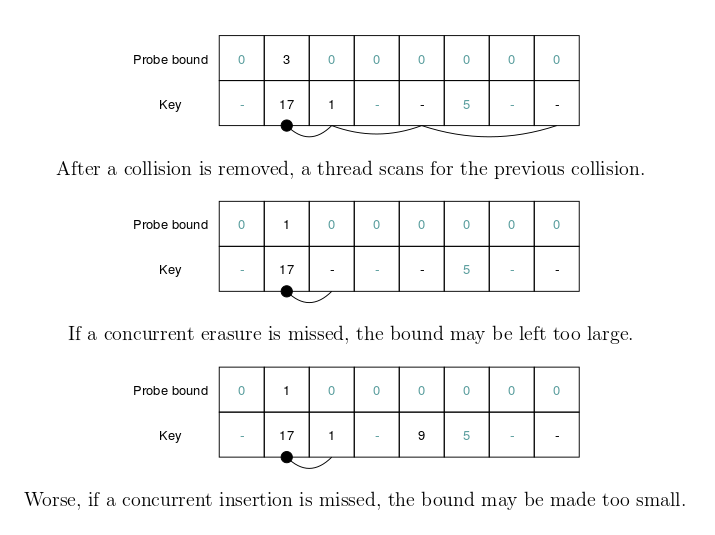
\includegraphics[scale=0.5]{non_blocking_1.png}
\caption{Problems maintaining a shared bound, after a collision is removed from the probe sequence}
\label{non_blocking_1}
\end{figure}

For this reason, we add a scanning bit for each probe bound, that we are able to update atomically, along with the probe bound. During insertion, threads just attempt to clear the bit and increase the bound if necessary. During deletions, a thread that is trying to erase a collision uses this bit to make sure that no other concurrent  updates have been made and that the probe bound has decreased correctly.

Every individual bucket holds the value and a state variable that helps resolve conflicts and synchronize concurrent operations, as described later. In order to prevent the ABA  problem, a version count is integrated along with each state variable.

In order to perform an insertion, a thread takes the following steps: First, it finds an empty bucket, stores the value and sets the state of that bucket to inserting. Then , it scans the probe sequence, looking for other threads inserting the same key, or a completed insertion of that key  ( characterized with the state member) . If a completed insertion is found, the thread sets its own working bucket to empty and the operation fails. If any other unfinished insertion operations are detected, the thread assists in the process of setting the first insertion found in the process to member and setting all the rest to collided. This operation is done concurrently by all threads working on the probe sequence, resulting in a lock –free algorithm where the delay of a single thread will not stall the others.

The main outline of the Insert and Assist operations are shown bellow.

\begin{lstlisting}[caption={Insert and Assist operation of the non blocking open addressing algorithm}]

bool Insert(int key){
	h = Hash(k)
	i=-1
	do
		if ++i>= size 
			table is full
		<version, state> = Bucket(h,i)->vs
	while (! CAS (&Bucket(h,i)->vs,<version, empty>,<version, busy>))
	Bucket(h,i)->key=key
	while (!) {
		Bucket(h,i)->vs = <version, visible>
		ConditionallyRaiseBound(h,j)
		Bucket(h,i)->vs = <version, inserting>
		r = Assist(k,h,i,version)
		if Bucket(h,i).vs != <version, collided>
			return true
		if !r
			ConditionallyLowerBound(h,i)
			Bucket(h,i)->vs = <version+1, empty>
			return false
		version ++
	}
}

bool Assist(int k, int h, int i , int ver_i){
	max = GetProbeBound(h)
	for (j=0; j<max ;j++){
		if i!=j {
			<ver_j,state_j> = Bucket(h,j)->vs
			if state_j = inserting && Bucket(h,j)->key = k {
				if j<i{
					if Bucket(h,j)->vs = <ver_j,inserting){
					CAS(&Bucket(h,i)->vs, <ver_i,inserting>, <ver_i,collided>)
					return Assist(k,h,j,ver_j)
					}
				}else{
					if Bucket(h,i)->vs = <ver_i,inserting>
						CAS(&Bucket(h,j)->vs, <ver_j,inserting> ,<ver_j,collided>)
				}
			}
			<ver_j, state_j> = Bucket(h,j)->vs
			if state_j =  member && Bucket(h,j)->key = k{
				if Bucket(h,j)->vs = <ver_j, member>{
					CAS(&Bucket(h,i)->vs, <ver_i,inserting>,<ver_i, collided>)
					return false
				}
			}
		}
	CAS(&Bucket(h,i), <ver_i, inserting>, <ver_i, member>)
	return true
}

					
						
\end{lstlisting}

Figure \ref{non_blocking_2} is an example of how the algorithm detects and avoids collisions.

 %figure 9 apo paper
\begin{figure}
 \centering
  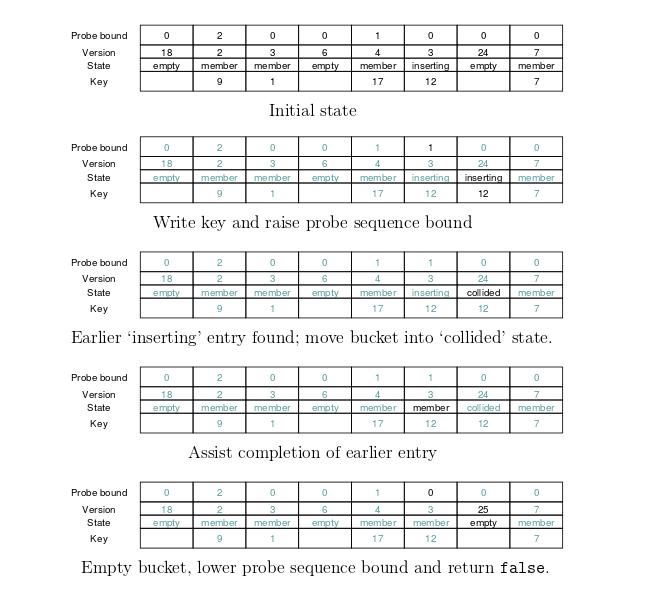
\includegraphics[scale=0.5]{non_blocking_2.png}
\caption{Inserting 12 using the lock-free algorithm.}
\label{non_blocking_2}
\end{figure}

The impact of the ABA problem is better understood from the following example of bad synchronization between inserting threads, in figure \ref{non_blocking_3} , that can be avoided with the use of version counters.

%figure 7 apo paper
\begin{figure}
 \centering
  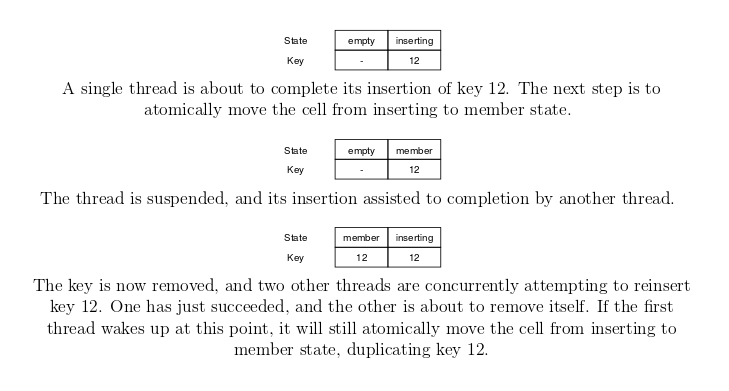
\includegraphics[scale=0.5]{non_blocking_3.png}
\caption{The effect of the ABA problem on concurrent assisting of operations.}
\label{non_blocking_3}
\end{figure}

This open addressing algorithm also requires bigger, partialy empty hash tables and resizing is again slow. However, if we know the aproximate size of the values inserted in advance, or if the workload consists mainly of lookups while instertions are rare, this implementation may perform better than the others,  mainly due to low it's small cache footprint that works very well with NUMA architectures. Figure \ref{hashes_non_blocking_perf} demonstrates that behaviour.

\begin{figure}
 \centering
  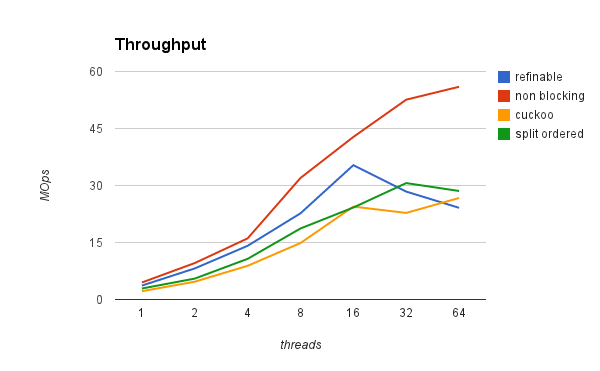
\includegraphics[scale=0.5]{hashes_non_blocking_perf.png}
\caption{Performance of the non blocking open addressing implementation}
\label{hashes_non_blocking_perf}
\end{figure}

\section{Transactional memory}

For completeness, we also present a simple implementation using hardware transactional memory on Intel's Hashwell multiprocessor. Operations on the table are executed inside a transcation. After a few consequtive aborts, a global lock is used as a fallback mechanism.

Figure \ref{hashes_tsx_perf} suggests that the transactional memory implementation perform very well, only when the workload consists only by lookups.In that case threads, dont modify memory locations and the absence of locking overhead leads to good performance. However, even a small percentage of insertions cause a significant amount of aborts and the advantage of transactional memory is quickly lost. In fact, as insertions become a bigger porportion of the workload, more and more transcation use the fallback mechanism and the algorithm gradually degrades down to the naive global lock aproach.

\begin{figure}
 \centering
  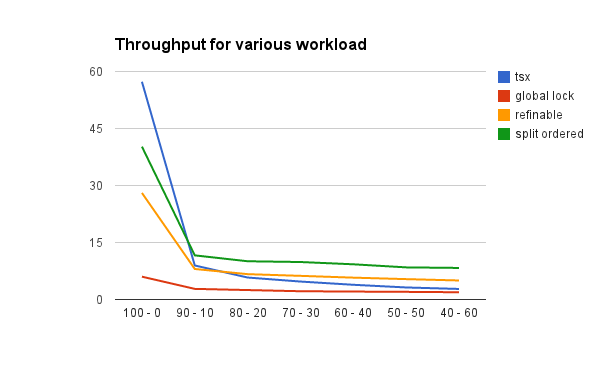
\includegraphics[scale=0.5]{hashes_tsx_perf.png}
\caption{Performance of various implementations as the workload changes}
\label{hashes_tsx_perf}
\end{figure}
